% Created 2018-06-21 Thu 12:30
\documentclass[8pt]{beamer}
\usetheme{Montpellier}
\usecolortheme{dove}

\usepackage[utf8]{inputenc}
\usepackage[T1]{fontenc}
\usepackage{fixltx2e}
\usepackage{graphicx}
\usepackage{longtable}
\usepackage{float}
\usepackage{wrapfig}
\usepackage{rotating}
\usepackage[normalem]{ulem}
\usepackage{amsmath}
\usepackage{textcomp}
\usepackage{marvosym}
\usepackage{wasysym}
\usepackage{amssymb}
\usepackage{hyperref}
\tolerance=1000
\usetheme{default}
\author{Siddharth Bhat}
\date{June 22nd, 2018}
\title{Counting integer points in polyhedra}
\hypersetup{
  pdfkeywords={},
  pdfsubject={},
  pdfcreator={Emacs 24.5.1 (Org mode 8.2.10)}}
\begin{document}

\maketitle

\begin{frame}[label=sec-1]{Definitions}
\begin{itemize}
\item Polyhedra: $\Big\{ \vec{x} \in \mathbb{Q}^d \mid Ax \leq \vec{b} \Big\}$
\item Polytope: bounded polyhedra.
\item Cone: $cone(\vec{u_i}) = \Big\{ \sum_i \lambda_i \vec{u_i} \mid \lambda_i \geq 0 \Big \}$, $\vec{u_i} \in \mathbb{Q}^d$
\item Simple cone: $SK = cone(\vec{u_i}), \vec u_i \in \mathbb{Z}^d$, $\vec u_i$ are linearly independent.
\item Unimodular cone: $UK = cone(\vec u_i)$, $Volume(\vec u_i) = 1$
\item Line: subspace.
\end{itemize}
\end{frame}

\begin{frame}[label=sec-2]{Pictures of defintions!}
\begin{itemize}
\item polytope
\end{itemize}
\begin{center}
 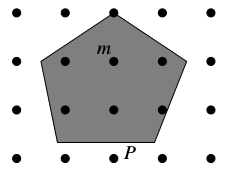
\includegraphics[width=1cm, keepaspectratio]{res/polytope}
\end{center}

\begin{itemize}
\item cone
\end{itemize}
\begin{center}
 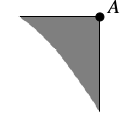
\includegraphics[width=1cm, keepaspectratio]{res/cone}
\end{center}

\begin{itemize}
\item polyhedra
\end{itemize}
\begin{center}
 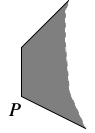
\includegraphics[width=1cm, keepaspectratio]{res/polyhedra}
\end{center}
\end{frame}

\begin{frame}[label=sec-3]{Example 1: valuation of line}
\begin{itemize}
\item P is a polyhedra, then $\mathcal{F}([P]) = \sum_{\vec{m} \in P \cap \mathbb{Z}^d} (x^{\vec{m}} )$
\item $\mathcal{F}([P])(\vec 1)$ = number of points.
\end{itemize}
\begin{align*}
\mathcal{F}((-\infty, \infty)) &= \sum_{i \in \mathbb{Z}} x^i \\
\text{count}(x) &= \mathcal{F}((-\infty, \infty)) \\
                &= \mathcal{F}((-\infty, 0]) + \mathcal{F}([0, \infty))  - \mathcal{F}(0) \\ 
                &=( \ldots + x^{-2} + x^{-1} + x^0) + (x^0 + x^1 + x^2 + \ldots) - x^0 \\
                &= \frac{1}{1 - \frac{1}{x}} + \frac{1}{1 - x} - 1 \\ 
                &= \frac{-x}{1 - x} + \frac{1}{1 - x}  = \frac{1 - x}{1 - x} - 1 = 0 \\
\end{align*}

\begin{itemize}
\item number of points in a line is 0!
\end{itemize}
\end{frame}
\begin{frame}[label=sec-4]{Example 2: valuation of interval}
\begin{center}
 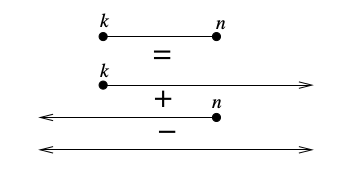
\includegraphics[width=3cm, keepaspectratio]{res/interval}
\end{center}

\begin{align*}
\text{count}(x) &= \mathcal{F}([0, n]) = \mathcal{F}([k, \infty)) + \mathcal{F}((-\infty, n]) - \mathcal{F}((\infty, infty)) \\
                &= (x^k + x^{k + 1} + \ldots) + \\
                & (\ldots +  x^{n - 2} + x^{n - 1} + x^n) +  \\
                & (\ldots + x^{-2} + x^{-1} + x^0 + x^1 + \ldots) \\
                &= \frac{x^k}{1 - x} + \frac{x^n}{1 - x^{-1}} + 0 \\
                &= \frac{x^k - x^{n + 1}}{1 - x} \\
\text{count}(1) &= \text{L'hospital} = (n + 1) - k = n - k + 1
\end{align*}
\end{frame}


\begin{frame}[label=sec-5]{Proof outline}
\begin{itemize}
\item Algbra of polyhedra, $P(\mathbb{Q}^d)$
\item $[\text{ }] : \mathbb{Q}^d \rightarrow P(\mathbb{Q}^d)$
\item Existence of $\mathcal{F}: P(\mathbb{Q}^d) \rightarrow \mathbb{C}(x)$, such that:
\begin{itemize}
\item \mathcal{F} is linear
\item P is a polyhedra, then $\mathcal{F}([P]) = \sum_{\vec{m} \in P \cap \mathbb{Z}^d} (x^{\vec{m}} )$
\item $\mathcal{F}([\text{line}]) = 0$ (important, allows modulo line decompositions)
\end{itemize}
\item $\mathcal{F}(P)(1) = \text{number of points in} P$
\item reduction: \mathcal{F} for cones gives full \mathcal{F}
\item reduction: \mathcal{F} for simple cones gives \mathcal{F} for cones
\item performance: $\mathcal{F}$ for unimodular cones gives $\mathcal{F}$ for simple cones
\end{itemize}
\end{frame}


\begin{frame}[label=sec-6]{Caveats}
\begin{itemize}
\item Self taught :)
\item Do not understand subtleties of convergence arguments (how is evaluating at $\vec{1}$ correct?).
\item No intuition for LLL, Lattice reduction.
\end{itemize}
\end{frame}



\begin{frame}[label=sec-7]{Assuming $\mathcal{F}$ for cones, derive full $\mathcal{F}$: Part 1 (Polytopes)}
\begin{center}
 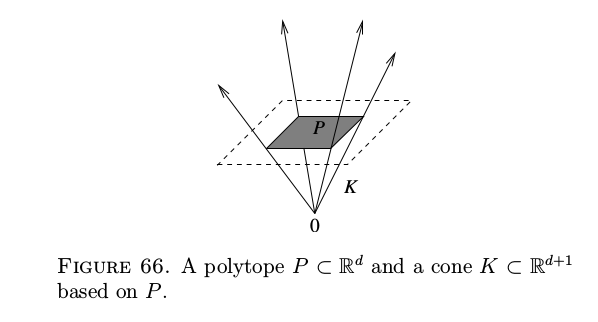
\includegraphics[width=6cm, keepaspectratio]{res/polytope-as-cross-section-of-cone}
\end{center}
\begin{itemize}
\item Write polytope as intersection of hyperplane + cone.
\item $\mathcal{F}(\text{polytope}) = (\frac{d}{dx_{d+1}} \mathcal{F}(\text{cone}))(\langle \vec 1^{d}, 0 \rangle)$
\item $\mathcal{F}(\text{cone}) = {x_{d+1}}^0 (\ldots) +  {x_{d+1}} (\texttt{POLYTOPE}) +  {x_{d+1}}^2(\ldots) + \ldots$
\item $\frac{d}{dx_d} \mathcal{F}(\text{cone}) = 0 + 0 \cdot  (\ldots) + 1 \cdot \texttt{POLYTOPE} +    2 x_{d+1} (\ldots) + \ldots$
\item $\frac{d}{dx_d} \mathcal{F}(\text{cone})(\langle \vec 1^{d}, 0 \rangle) = \texttt{POLYTOPE(\(\vec 1 \))} +  2 \cdot 0 \cdot (\ldots) + \ldots$
\item $\frac{d}{dx_d} \mathcal{F}(\text{cone})(\langle \vec 1^{d}, 0 \rangle) = \texttt{POLYTOPE(\(\vec 1 \))}$
\end{itemize}
\end{frame}




\begin{frame}[label=sec-8]{Assuming $\mathcal{F}$ for cones, derive full $\mathcal{F}$: Part 2 (Lines)}
\begin{itemize}
\item Line = $\sum$$_{\text{dimension}}$ cone + cone - point.
\item Since line can be translated:
\end{itemize}
\begin{align*}
\forall \vec{x} \in L, L &= \vec{x} + L \\
\forall x \in L, \mathcal{F}(L) &= \mathcal{F}(L) + \mathcal{F}(\vec{x})  \\
\mathcal{F}(L) &= 0 \\
\end{align*}

\begin{align*}
\text{count}(x) &= \mathcal{F}((-\infty, \infty)) \\
                &=( \ldots + x^{-2} + x^{-1} + x^0) + (x^0 + x^1 + x^2 + \ldots) - x^0 \\
                &= \frac{1}{1 - \frac{1}{x}} + \frac{1}{1 - x} - 1 \\ 
\end{align*}
\begin{itemize}
\item In 1-d example, radius of convergence of left and right cone was 0
\item Is this really well-defined? (what is this ring which admits $f(x) = \ldots + x^{-1} + x^0 + x^1 + \ldots$)
\end{itemize}
\end{frame}


\begin{frame}[label=sec-9]{Assuming $\mathcal{F}$ for simple cone, derive for cone}
\begin{itemize}
\item Simple cone: $SK = co(u_i) = \{ \sum_i \lambda_i u_i \vert \lambda_i \geq 0 \}$, $u_i \in \mathbb{Z}^d$, $u_i$ are linearly independent.
\item Cone: $C = co(u_i)$, $u_i \in \mathbb{Q}^d$
\item inclusion exclusion: decompose cone into simple cones.
\end{itemize}
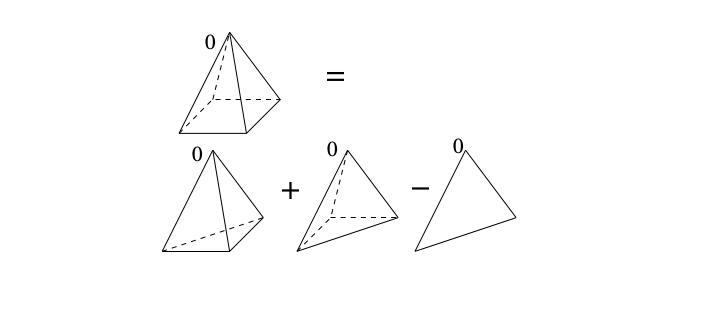
\includegraphics[width=.9\linewidth]{./res/cut-cone-into-simple-cones.png}
\end{frame}


\begin{frame}[label=sec-10]{$\mathcal{F}$ for simple cones: Part 1}
\begin{itemize}
\item Consider the positive orthant in 3D: $P \subset \mathbb{Q}^3 = \Big\{(x, y, z) \mid x, y, z \geq 0 \Big\}$
\item $P = cone((1, 0, 0), (0, 1, 0), (0, 0, 1))$
\item this is a simple cone, and here's how we count it:
\end{itemize}

\begin{align*}
\mathcal{F}([P]) &= \sum_{i, j, k \in [0, \infty)} x^i y^j z^k \\
                 &= \sum_{i=0}^\infty x^i \Bigg(\sum_{j=0}^\infty y^j \Bigg(\sum_{k=0}^\infty z^k\Bigg)\Bigg) \\
                 &= \frac{1}{1 - x} \cdot \frac{1}{1 - y} \cdot \frac{1}{1 - z}
\end{align*}
\end{frame}


\begin{frame}[label=sec-11]{$\mathcal{F}$ for simple cones: Part 2}
\begin{itemize}
\item General story is similar
\item $SK = co(u_i)$, $u_i$ linearly independent.
\item Since $u_i$ is linearly independent, some points $\vec{x} \in cone(u_i)$ have unique representation  $\vec x = \sum_i \lambda_i u_i$, $\lambda_i \in \mathbb{Z}$
\item fundamental paralellopiped $(\Pi)$ will tile the plane.
\item We can count the $\vec{x}$, and make $\vec{x}$ responsible for the "tile" of skipped points.
\end{itemize}

\begin{center}
 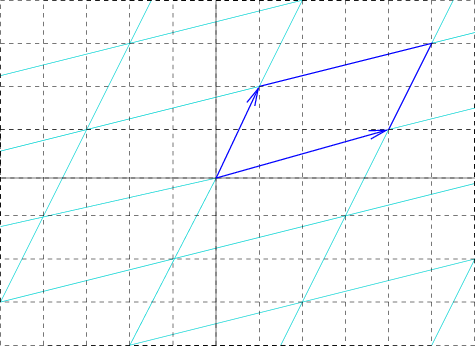
\includegraphics[width=3cm, keepaspectratio]{res/fundamental-paralellopiped-tiled}
 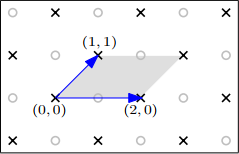
\includegraphics[width=3.40cm, keepaspectratio]{res/fundamental-parallelopiped.png}
\end{center}

$$\mathcal{F}(SK) &= \Bigg(\underbrace{\sum_{\vec p \in \Pi \cap \mathbb{Z}^d} x^{\vec p} }_\text{per-tile points} \Bigg)
                           \underbrace{\prod_i \frac{1}{1 - x^{u_i}}}_\text{tile starting point \( \vec{x} \)}$$
\end{frame}

\begin{frame}[label=sec-12]{Performance - How?}
\begin{itemize}
\item Write simple cone as sum of unimodular cones:
\end{itemize}
$$[K] = \sum_i \alpha_i [K_i]+ \text{lower dimesnional cones}$$ 

\begin{itemize}
\item We concentrate on $\sum_i \alpha_i [K_i]$
\end{itemize}
\begin{center}
    $\alpha_i \in \{ -1, 1 \}$  and $K_i$ are unimodular.
\end{center}

\begin{itemize}
\item Lower dimensional cones are taken care of by a trick.
\end{itemize}
\end{frame}



\begin{frame}[label=sec-13]{Unimodular decomposition of a simple cone $K$: Part 1}
\begin{center}
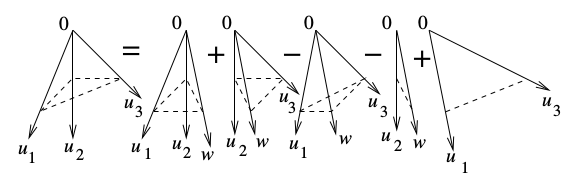
\includegraphics[width=10cm, keepaspectratio]{res/simple-cone-into-unimodular-cones}
\end{center}
\end{frame}

\begin{frame}[label=sec-14]{Unimodular decomposition of simple cone $K$: Part 2}
\begin{itemize}
\item $Index(K) = Volume(\Pi(K))$
\end{itemize}

$Index(K) = 1 \leftrightarrow \text{K is unimodular}$. $Index(K)$ is a measure of non-unimodularity.

\begin{itemize}
\item Introduce procedure which takes \textbf{polynomial steps} to \textbf{reduce Index(K)}
\item Let $K = cone(u_1, u_2, \ldots, u_d)$, $u_i \in \mathbb{Z}^d$, $u_i$ are linearly independent.
\item High level idea:
\begin{itemize}
\item Pick a non-zero integer point $p$, which is shorter than the current $u_i$.
\item create $d$ new "basis sets", $\texttt{Basis}_j = \{u_1, u_2 , \ldots, u_d\} \setminus \{u_j\} \cup \{p\}$
\item make new cones, $K_i = cone(\texttt{Basis}_j)$ and show that $Index(K_i) < Index(K)$
\item Intuition for shorter index: $p$ is shorter than $u_i$, parallelopiped will be smaller.
\item $K = \sum \alpha_i K_i + \text{faces of \(K_i \)}$
\item show that $Index(K_i)$ reduces by a large enough factor that poly rounds are enough to reduce to 1
\item eliminate faces for $K_i$ with trick to kill lower dimensional objects.
\end{itemize}
\end{itemize}
\end{frame}

\begin{frame}[label=sec-15]{Decomposition example}
\begin{center}
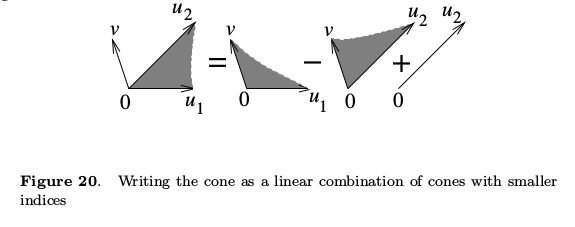
\includegraphics[width=7cm, keepaspectratio]{res/simple-cone-as-combination-smaller-indeces}
\end{center}
\end{frame}


\begin{frame}[label=sec-16]{Polar trick}
\begin{itemize}
\item Polar: $$P^\circ = \Bigg\{ \vec y \in \mathbb{Q}^d :  \forall \vec p \in P, \  \vec p \cdot \vec y  \ \geq 0 \Bigg\}$$
\end{itemize}

\begin{center}
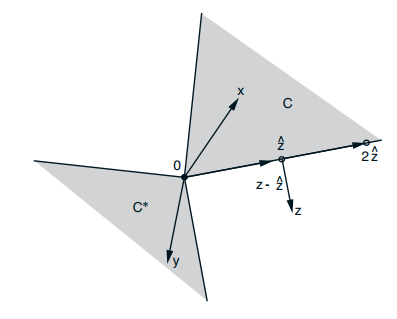
\includegraphics[width=3.40cm, keepaspectratio]{res/polar-of-cone.png}
\end{center}

\begin{itemize}
\item Lower dimensional cones do not matter. First take $[K^\circ]$, then compute unimodular decomposition of this:
\end{itemize}
$$[K^\circ] = \sum_i \alpha_i [K_i] + \text{lower dimensional cones}$$
$$[(K^\circ)^\circ] = [K] = \sum_i \alpha_i K_i + \text{cones with lines}$$
$$ \mathcal{F}([K]) = \sum_i \alpha_i \mathcal{F}(K_i) + \mathcal{F}(\text{cones with lines}) = \sum_i \alpha_i \mathcal{F}(K_i) + 0$$
\end{frame}



\begin{frame}[label=sec-17]{References}
\begin{itemize}
\item Lattice Points, Polyhedra, and Complexity: Alexander Barvinok
\item Integer points in polyhedra: Alexander Barvinok
\end{itemize}
\end{frame}


\begin{frame}[label=sec-18]{Thanks!}
Questions?
\end{frame}


\begin{frame}[label=sec-19]{Minkowski convex body theorem}
\begin{itemize}
\item Statement: Convex set $P \subset \mathbb{R}^d$, which is symmetric with respect to the origin ($\forall x \in P, -x \in P$), has volume greater than or
equal to $2^d$ contains a non-zero integer point.

\item Recap: Let $K = cone(u_1, u_2, \ldots, u_d)$, $u_i \in \mathbb{Z}^d$, $u_i$ are linearly independent.
\begin{itemize}
\item Pick a non-zero integer point $p$ in $K$ \textbf{(why does this integer point exist?)}.
\end{itemize}

\item Construct $$\Pi_0 = \Bigg\{ \sum_i \alpha_i u_i :  |\alpha_i| \leq \frac{1}{\sqrt[d]{Index(K)}}  \Bigg\}$$
\begin{itemize}
\item Symmetric
\item Length per axis: $\frac{2 |u_i|}{\sqrt[d]{Index(K)}}$
\end{itemize}

\item Total volume:
\end{itemize}
\begin{align*}
Volume(\Pi_0) &= \prod_{i=1}^d \frac{2 |u_i|}{\sqrt[d]{Index(K)}}\\
 &= 2^d \frac{ \prod_{i=1}^d |u_i| }{Index(K)} = 2^d
\end{align*}

\begin{itemize}
\item Hence, by Minkowski convex body, we find a point $p \in \mathbb{Z}^d$ in $\Pi_0$. If this point is in the wrong direction (facing outward), pick $-p$.

\item This only gives us \textbf{existence} of such a point; need to use LLL to \textbf{construct} this point.
\end{itemize}
\end{frame}

\begin{frame}[label=sec-20]{Minkowski convex body theorem example}
\begin{center}
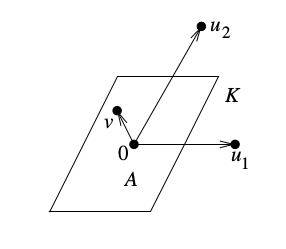
\includegraphics[width=3cm, keepaspectratio]{res/minkowski-convex-body}
\end{center}
\end{frame}


\begin{frame}[label=sec-21]{LLL  (Lenstra–Lenstra–Lovász lattice basis reduction)}
\begin{itemize}
\item Given an arbitrary basis $u_i \in \mathbb{Z}^d$ of a lattice, produces a new basis which is "nicer".
\item New basis consists of shorter vectors that are "more orthogonal"
\item Runs in polynomial time.
\item Determining \textit{shortest basis} is hard - used in cryptosystems IIUC.
\end{itemize}

\begin{center}
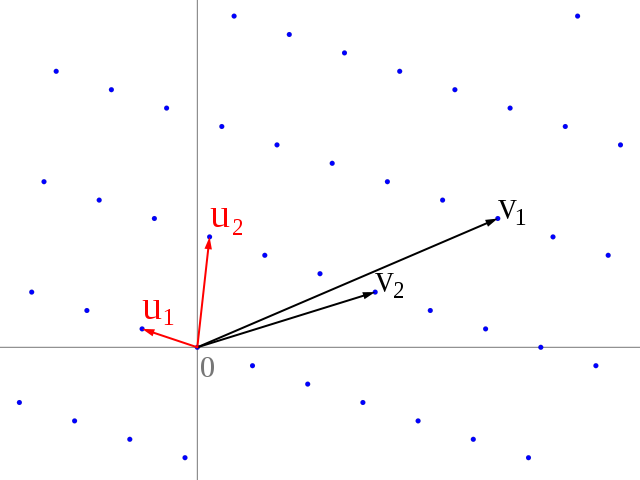
\includegraphics[width=7cm, keepaspectratio]{res/lattice-reduction}
\end{center}
\begin{itemize}
\item Black is input, red is output.
\end{itemize}
\end{frame}


\begin{frame}[label=sec-22]{Using LLL}
\begin{itemize}
\item Refer to page $140$ of integer points in polyhedra.

\item Recap: Let $K = cone(u_1, u_2, \ldots, u_d)$, $u_i \in \mathbb{Z}^d$, $u_i$ are linearly independent.
\begin{itemize}
\item Pick a non-zero integer point $p$ in $K$ \textbf{(how do we find it?)}
\end{itemize}

\item Let $T: V \rightarrow V$, $T(u_i) = e_i$.
\item Let $\Lambda  = \text{Lattice of } u_i$
\item $\Lambda_0 = T(\Lambda)$
\item Apply LLL on $\Lambda_0$, get shorter description
\item Construct $w_0 \in \Lambda_0 \setminus \{ 0 \}$ such that $\lVert w_0 \rVert_{\infty}$ is minimum.
\item This bounds $\lVert w_0 \rVert  \leq \lVert w_0 \rVert_{\infty} \sqrt{d}$ .
\item $w = T^{-1}(w_0)$
\end{itemize}



\begin{itemize}
\item Caveat: Why do we need this song and dance? Why not just work on the original space?
\end{itemize}
\end{frame}

\begin{frame}[label=sec-23]{Assuming $\mathcal{F}$ for cones, derive full $\mathcal{F}$: Part 1.2 (Polytopes)}
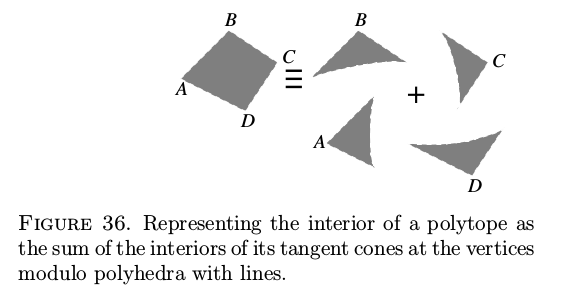
\includegraphics[width=.9\linewidth]{./res/polytope-as-sum-of-tangent-cones.png}
\end{frame}
% Emacs 24.5.1 (Org mode 8.2.10)
\end{document}
